\section{Interpretation Methods}
\label{sec:interpretation_methods}

There exists a variety of definitions in the vastly expanding research field of XAI, and the concept of \textit{interpretability} still has no formal commonly used technical meaning \cite{lipton2018mythos}. To build on the common ground of existing research, this work follows the terminology of Lipton et al. \cite{lipton2018mythos} and Arrieta et al. \cite{arrieta2020explainable}.

Broadly, interpretability focuses on \textit{how} and \textit{why} a machine learning model makes predictions.
Simply put, interpretability is focused on getting some notion of an explanation in human understandable terms for the decisions made by a machine learning model.

%%%%%%%%%%%%%%%%%%%%%%%%%%%%%%%%%%%%%%%%%%%%%%
\subsection{Terminology}
\label{subsec:interpretation_methods_terminology}
The authors of \cite{arrieta2020explainable} make a distinction between the related but different concepts of \textit{interpretability} and \textit{explainability}. Lipton \cite{lipton2018mythos} further breaks down interpretability into \textit{transparency} and \textit{post-hoc} interpretability. The notion of \textit{explainability} from \cite{arrieta2020explainable} can be related to Liptons's \textit{transparency}, while Lipton's \textit{post-hoc} interpretability is essentially \textit{interpretability} as defined by Arrieta et al. \cite{arrieta2020explainable}.

\mypar{Post-hoc Interpretability} refers to the the extent to which cause and effect can be observed in a model, which can be translated to uncovering \textit{why} a model made prediction $y$ to an input $\mathbf{x}$, or how input and output relate to each other. \textit{Post-hoc} means that interpretations are computed by applying methods that analyze the model after training. Consider the example of image classification from \autoref{fig:bb}. Here, interpretability would mean that if a cat is present in the image (the cause), the (trained) model classifies it to the category 'cat' (the effect). Now imagine we find that the model takes the green meadow in the image as evidence to predict 'cat', and not the cat itself. This would imply a lack of interpretability, as the model learns to assign features to the concept 'cat' other than those related to 'cat' in the correct sense. This toy example emphasizes a common problem in image classification: \cite{xiao2020noise} observe the over-reliance of models on image background, rather than on objects in the foreground, and is thus not just a reality distant toy example.

\mypar{Explainability or Transparency} on the other hand spans methods to uncover \textit{how} a model makes predictions, meaning to observe the inner workings of a model and thus to literally explain what is happening in terms of understanding of the mechanisms by which a model works. Thus, transparency refers to the model's inherent properties that can be known before the training process and that are helpful to understand the model.

\par\smallskip\vspace*{-0.1cm}
While both concepts seem to be important for the general objective of explainable artificial intelligence, this paper focuses on post-hoc interpretability.
There are essentially two ways to achieve interpretability: (1) to use inherently interpretable models or (2) to post-process a model in a fashion that allows to yield insights into it's decision. 
An inherently interpretable model is a model with restricted complexity (e.g. a linear model). On the other hand, \textit{post-hoc}, as outlined earlier, refers to the application of methods for analyzing a model after model training.
Post-hoc methods span \textit{model-agnostic} methods and \textit{model-transparent} methods. Within model-agnostic methods, the model itself is unknown and approximated with a \textit{surrogate} model (see \autoref{subsec:bb_methods}), while within \textit{model-transparent} methods, the model itself is used to compute interpretations (see \autoref{subsec:wb_methods}). 

\mypar{Local and Global Methods.} A further categorization can be made based on the scope of interpretations: \textit{Local} methods aim at providing interpretations that are true for a single data point and its neighbors. 
\textit{Global} methods aim at gaining interpretations that are valid for most data points in a class \cite{kim2018interpretability, nguyen2017plug, yosinski2015understanding}. The interpretation methods discussed within this paper mostly fall into the class of local explanation methods \cite{ribeiro2016should, lundberg2017unified, bach2015pixel}.

\mypar{Feature Attribution Methods and Sample Attribution Methods. } Interpretation methods aim at making complex and inherently uninterpretable black box models interpretable by creating human readable visualizations. 
A frequently used type of explanation methods are \textit{feature attributions} mapping each input feature to a numeric score. This score should quantify the importance of the feature relative to the model output. The resulting attribution map is then visualized as a heatmap projected onto the input sample. This allows humans to interpret which input attributes are the most helpful for making tha final prediction. Sample attribution methods on the other hand interpret the model performance in terms of the importance of training examples from the dataset. 

We adhere to the following formal definition of an interpretation method:\newline

\textbf{Definition 1: Interpretation Method.}

\setlength{\leftskip}{0.39cm}

  \noindent We consider a neural network $N: \mathbb{R}^d \to \mathbb{R}^k$. For the an arbitrary classification task, $N$ classifies an input sample $\mathbf{x}\in \mathbb{R}$ in $k$ categories where the prediction $f_N(\mathbf{x})=y \in \{1, ..., K\}$ is given by $y = arg max_i f_N(\mathbf{x})_i$.

  Given the neural network $N$, it's input vector $\mathbf{x} \in \mathbb{R}^d$ and the the neural networks prediction for input $\mathbf{x}$, $f_N(\mathbf{x})=y$, an interpretation method $\mathcal{I}$ determines why label $y$ has been chosen by $N$ for input $\mathbf{x}$. 
  The interpretation is given by an output vector $\mathbf{h_k} \in \mathbb{R}^d$ for a class $k$ where each entry $h_i$ is mostly a numeric value describing the relevance for the $i$-th input feature $x_i$ of $\mathbf{x}$ for the final score $f_N(\mathbf{x})$.

\setlength{\leftskip}{0pt}
\par\smallskip\vspace{-0.1cm}

As $\mathbf{h}$ has the same dimensions as the input $\mathbf{x}$ it can be mapped to the input, overlaying $\mathbf{x}$ as a heatmap, where the color value represents the importance of feature $x_i$ towards the prediction $f_N(\mathbf{x})$.
An example is given in \autoref{fig:lrp_cat_lrp}. Higher values, implying a stronger relative importance for making the prediction $f_N(\mathbf{x})$, are depicted in dark red. 

While all explanation methods try to obtain importance measures for the network prediction, they differ with respect to how these measures are obtained. \cite{evaluating_explanations_security} propose two major categories for interpretation strategies, namely \textit{black-box}, in the following named \textit{model-agnostic} methods and \textit{white-box}, or \textit{model-transparent} interpretation methods. 
While black-box interpretations assume no knowledge about the underlying model, white-box methods only work by using the model parameters. 

This terminology of discriminating between black-box and white-box methods may not be confused with the nature of the underlying models: Models still remain of black-box nature even though a white-box method may contribute to making the decision making process of such a model more insightful.

The following section details the two categories and gives examples of commonly used interpretation methods within each group. 

\subsection{Model-agnostic methods.}
\label{subsec:bb_methods}

% https://proceedings.neurips.cc//paper/2020/file/2c29d89cc56cdb191c60db2f0bae796b-Paper.pdf p. 4 
Model-agnostic interpretations assume no knowledge about the model thus treating it as a black box. The underlying model is approximated by learning it's behavior with an interpretable model, e.g. a linear model. The interpretable model is also dubbed the 'surrogate' model. The common approach for learning the surrogate is to approximate the relationship between the input samples and the corresponding prediction by the model.
As the model itself does not need to be known, these approaches can be used in scenarios where the model itself is not directly accessible. Model-agnostic interpretations are fairly popular and are used in a wide range of applications, ranging from finance and law to medicine and chemistry \cite{elshawi2019interpretability, whitmore2016mapping}. 

A black-box interpretation offers the great advantage of being applicable to any model and offers simplicity because the interpretation is embedded in the model. However, this option of gaining interpretability might be costly for users that already have a high performing model. For this reason, growing need for methods exists that can be applied without retraining or modifying the underlying model.
We will briefly describe two common model-agnostic approaches. Please refer to the original papers for details.

\mypar{Local Interpretable Model-agnostic Explanations (LIME).}\newline
LIME \cite{ribeiro2016should} perturbs the input and observes how the predictions of a black box model change. For the task of image classification, LIME creates a set of perturbed instances by dividing the input image into interpretable components, which are technically contiguous super-pixels, and runs each perturbed instance through the model to get the probability for how much the change in each super-pixel influences the whole model prediction. 

\autoref{fig:lime_cat} shows an example of LIME applied to the neural network model Inception-v3 \cite{szegedy2016rethinking}. Input image from the ImageNet dataset \cite{ILSVRC15}. The super-pixel in dog instances place is highlighted in green, which correctly indicates that this super-pixel has a high influence on the prediction of the images correct class ('bernese mountain dog'). LIME also correctly indicates that the super-pixel in the cat's place does not indicate the correct class label.

\begin{figure}[ht]
  \centering
  \begin{subfigure}{0.32\linewidth}
    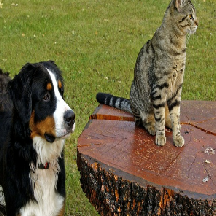
\includegraphics[width=\linewidth]{figures/lime_orig.png}
    \caption{Original}
    \label{fig:bird-a}
  \end{subfigure}
  \begin{subfigure}{0.32\linewidth}
    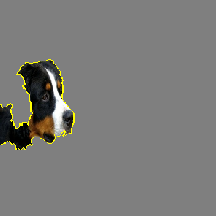
\includegraphics[width=\linewidth]{figures/lime_dog_mask.png}
    \caption{Mask.}
    \label{fig:bird-a}
  \end{subfigure}
  \begin{subfigure}{0.32\linewidth}
    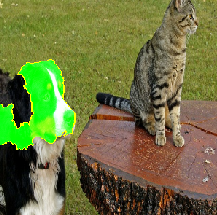
\includegraphics[width=\linewidth]{figures/lime_dog_map1.png}
    \caption{Saliency Map.}
    \label{fig:bird-a}
  \end{subfigure}
  \caption{Visualization of the output of the LIME interpreter applied to an image and image classification model.}\label{fig:lime_cat}
  \vspace{-0.3cm}
\end{figure}

% https://github.com/marcotcr/lime
% While the model may be very complex globally, it is easier to approximate it around the vicinity of a particular instance. While treating the model as a black box, we perturb the instance we want to explain and learn a sparse linear model around it, as an explanation. The figure below illustrates the intuition for this procedure. The model's decision function is represented by the blue/pink background, and is clearly nonlinear. The bright red cross is the instance being explained (let's call it X). We sample instances around X, and weight them according to their proximity to X (weight here is indicated by size). We then learn a linear model (dashed line) that approximates the model well in the vicinity of X, but not necessarily globally.

\mypar{SHapley Additive exPlanations (SHAP).} SHAP \cite{lundberg2017unified} builds on Shapley analysis, which is essentially about judging the importance of attributes. The model is trained on a number of subsets of all available features, and the feature importance scores are calculated by evaluating the effects that the omissions of the specific features have on the model prediction. An example is shown in \autoref{fig:shap_dog}. Image regions highlighted in green are found to be important for predicting the correct label.

\begin{figure}[ht]
  \centering
  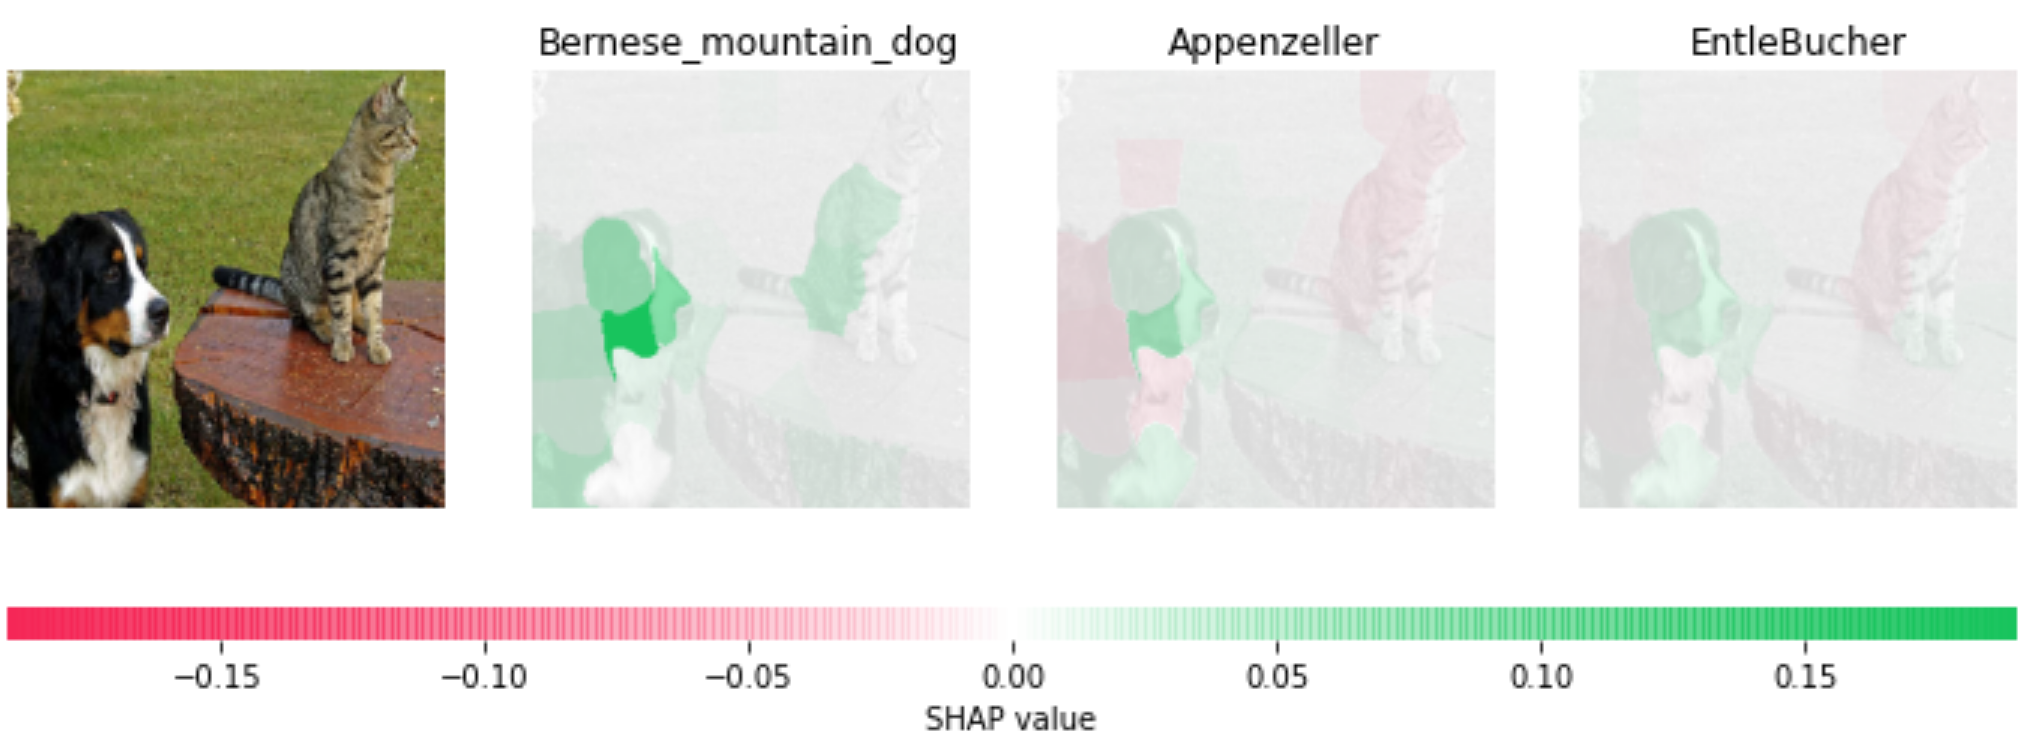
\includegraphics[width=\linewidth]{figures/cat_dog_shap.png}
  \caption{Visualization of the output of the SHAP interpreter applied to applied to an image and image classification model.}\label{fig:shap_dog}
  \vspace{-0.3cm}
\end{figure}

\subsection{Model-transparent methods.}
\label{subsec:wb_methods}

The other group of interpretations are model-transparent, or white-box methods, where the underlying model is known with all its parameters. Thus, the interpretation can be directly computed by using the model instead of relying on an approximation of $f_N$ as within the black-box methods. These methods typically rely on the relationship between an input sample, the underlying model's prediction and the associated activations of the models hidden layers. Methods within this group are for example propagation-based and gradient-based approaches. The former propagate the model's prediction back through the model. The latter make use of the information provided by the gradients of the loss function, which contain sensitive information about the prediction and the features. Using the backpropagation method, features in the input can be highlighted based on the amount of gradient they receive. This shows their contribution to the final score. 
A few example methods within this group are listed below. 

\mypar{Layer-wise Relevance Propagation (LRP).} While many approaches in the group of model-transparent interpretations are designed only for image classification, or convolutional neural networks, this method \cite{bach2015pixel} is an exception. LRP propagates relevance values backwards through the network and decomposes the score of a predicted class backwards through the network. It relies on a Taylor series close to the prediction point rather than partial derivatives at the prediction point itself. An example for a feature map produced by LRP can be found in \autoref{fig:lrp_cat_lrp}.
%The output is a heatmap of relevance values, depicting for each feature how helpful or harmful the feature is for predicting the target class. 

\mypar{DeepLIFT} \cite{shrikumar2017learning} is an improved version of LRP, where a reference point in the input feature space is defined. Relevance scores are propagated proportionally to the changes of neuronal activations from the reference. % https://arxiv.org/pdf/1710.10547.pdf

\mypar{SmoothGrad (SG)} \cite{smilkov2017smoothgrad} averages over interpretations of noisy copies of an input sample thus reducing noise by visually diffusing the interpretation. The noise is drawn i.i.d. from a normal distribution. 

Methods developed specifically for convolutional neural networks are for instance Grad-CAM \cite{selvaraju2017grad} or SimpleGrad \cite{simonyan2013deep}.

